\section{\graicore{}}

% One of these edge AI accelerators is the \graicore{} designed by GrAI Matter Labs (GML).
One of these edge AI accelerators is the \graicore{}.
The \graicore{} utilizes the ``NeuronFlow'' technology, a many-core architecture that is inspired by the neural structures of the brain \cite{moreiraNeuronFlowNeuromorphicProcessor2020}.
Its main use case is computer vision applications using models based on convolutional neural networks (CNNs).
It features a total of 144 neuron cores, arranged in a 12 by 12 grid.
A neuron core includes a local SRAM memory for storing data such as model parameters and a processing element for performing mathematical operations (see \cref{fig:neuron_core}).

\begin{figure}[htbp]
    \centering
    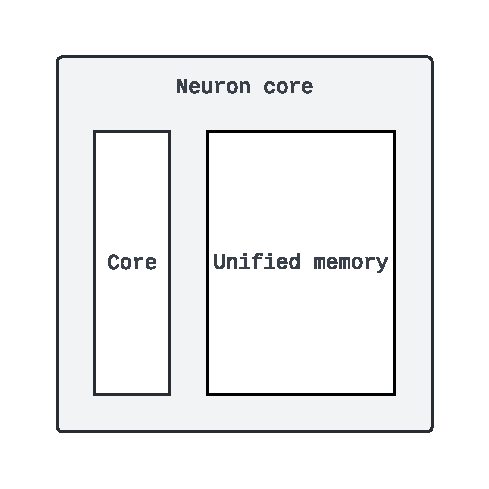
\includegraphics[width=0.25\textwidth]{assets/neuron_core.pdf}
    \caption{The neuron core includes a processing element (core) and a local memory (a.k.a. unified memory)}
    \label{fig:neuron_core}
\end{figure}

\subsection{Near-memory computing}
The \graicore{} makes use of near-memory computing.
Near-memory computing refers to an computer architecture where computation is performed close to the memory.
This approach aims to mitigate the ``von Neumann bottleneck'', a limitation caused by the traditional computing architecture where the CPU (Central Processing Unit) and memory are separate entities, and data must be transferred back and forth between them \cite{indiveriMemoryInformationProcessing2015}.
By performing computations closer to where data is stored, data movement between the processing element and memory is minimized, reducing latency and energy consumption.
However, this introduces a constraint that requires the parameters of a model to reside in local memory before it can be used by the processing element.
Thus, an AI model must first be mapped and loaded onto the \graicore{} before it can be used for inference.
Mapping means to assign the layers of a neural network to the neuron cores.
Intelligent mapping is important for balancing memory, computation and traffic between neuron cores.
The \graicore{} features a total of \SI{36}{MB} of local memory, which is evenly distributed across its $144$ neuron cores.
The size of an AI model can be quantified by the number of its parameters.
For instance, if a parameter is stored as a 16-bit value on the \graicore{}, it can accommodate approximately $\frac{\SI{36}{MiB}}{\SI{16}{b}}$ parameters\footnote{In practice, the available space for parameters is smaller because a portion of the memory is allocated for storing other relevant data.}, which translates to around \SI{19}{M} parameters in total.
Popular computer vision models like ResNet-50 \cite{heDeepResidualLearning2015} and YOLOv7 \cite{wangYOLOv7TrainableBagoffreebies2022}, with over \SI{25}{M} and \SI{37}{M} parameters respectively, are already too large by themselves to fit on the \graicore{}.
Using optimization techniques, these models can be compressed into a smaller size.
For example, YOLOv7-tiny \cite{wangYOLOv7TrainableBagoffreebies2022} is a size optimized model of the YOLOv7 for edge devices at the cost of accuracy.
Its size is decreased to around \SI{6}{M} parameters, making it suitable for the \graicore{}.
In summary, the number of parameters that can be stored on the \graicore{} is limited by the size of its memory.
% Due to this, the \graicore{} is only able to support limited sized AI models.

% TODO change to subcaption
\begin{figure}[htbp]
    \centering
    \subfloat[The \eventnoc{} features a 2D torus topology]{
        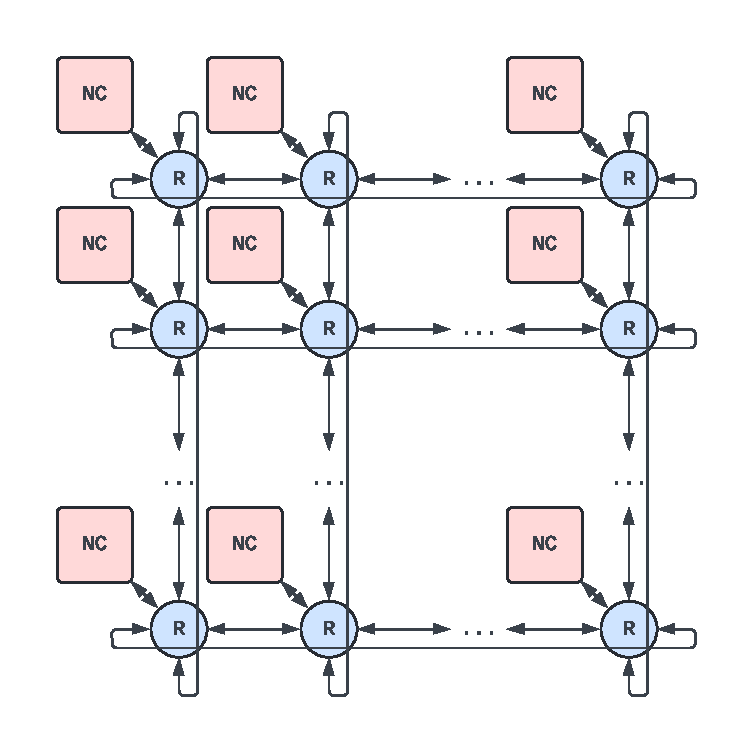
\includegraphics[width=0.45\textwidth]{assets/event_noc.pdf}
        \label{fig:event_noc}
    }
    \hfill
    \subfloat[The \confignoc{} features a 2D mesh topology]{
        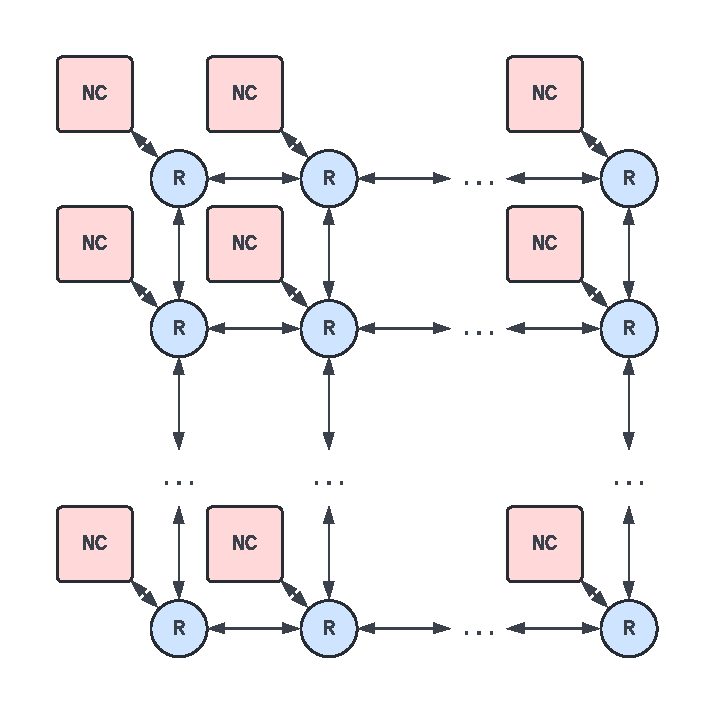
\includegraphics[width=0.45\textwidth]{assets/config_noc.pdf}
        \label{fig:config_noc}
    }
    \caption{\graicore{}'s network-on-chips. A neuron core (NC) communicates via its associated router (R) with other neuron cores and external parties such as the host device (not illustrated).}
    \label{fig:noc}
\end{figure}

\subsection{NoCs}
The neuron cores are connected to each other with two distinct network-on-chips (NoCs), each serving its own purpose (see \cref{fig:noc}).
% Firstly, the \eventnoc{} is responsible for transferring small packets of data called Events to its destination.
Firstly, the \eventnoc{} is used for exchanging activated neuron states in the form of small messages called Events.
Events are only generated when an AI model is being executed.
The \eventnoc{} uses the 2D torus topology.
Secondly, the \confignoc{} is responsible for configuring the \graicore{}, monitoring and debugging.
The \confignoc{} uses a different topology, namely a 2D mesh topology.
Configuring the \graicore{} means that the local memories of the neuron cores are written with the parameters of an AI model.
A host device (e.g., a microcontroller) initiates the configuration of the \graicore{}.
The host device is connected to the \confignoc{} via a single link, which is used to transfer data to and from any neuron core.
Since all data transfers must go through this link to reach its destination neuron core, it causes a significant bottleneck in data transfer speed to the \graicore{}.
That is, the amount of data that can be transferred to the neuron cores within a certain time is poor as it was not designed with speed in mind.
Therefore, currently, the configuration of the memories of the neuron cores is only performed once at the start.
% This limitation restricts the \graicore{} to be (partially) reconfigured at run-time.

